\documentclass[norsk,a4paper,12pt]{article}
\usepackage[utf8]{inputenc}
\usepackage{graphicx} %for å inkludere grafikk
\usepackage{verbatim} %for å inkludere filer med tegn LaTeX ikke liker
\usepackage{tabularx}
\usepackage{booktabs}
\usepackage{amsmath}
\usepackage{float}
\usepackage{color}
\usepackage{listings}
\usepackage{hyperref}
\usepackage{amsmath}
\usepackage{tikz}
\usepackage{physics}
\usepackage{amssymb}

\lstset{language=c++}
\lstset{basicstyle=\small}
\lstset{backgroundcolor=\color{white}}
\lstset{frame=single}
\lstset{stringstyle=\ttfamily}
\lstset{keywordstyle=\color{red}\bfseries}
\lstset{commentstyle=\itshape\color{blue}}
\lstset{showspaces=false}
\lstset{showstringspaces=false}
\lstset{showtabs=false}
\lstset{breaklines}
\lstset{postbreak=\raisebox{0ex}[0ex][0ex]{\ensuremath{\color{red}\hookrightarrow\space}}}
\usepackage{titlesec}

\setcounter{secnumdepth}{4}
\usetikzlibrary{through, shapes, calc, shapes, arrows, positioning}

\tikzstyle{neuron}=[draw,circle,minimum size=20pt,inner sep=0pt, fill=white]
\tikzstyle{stateTransition}=[thick]
\tikzstyle{learned}=[text=red]

\titleformat{\paragraph}
{\normalfont\normalsize\bfseries}{\theparagraph}{1em}{}
\titlespacing*{\paragraph}
{0pt}{3.25ex plus 1ex minus .2ex}{1.5ex plus .2ex}


\title{FYS4411 - Computational Physics II\\\vspace{2mm} \Large{Project 2}}
\author{\large Dorthea Gjestvang\\ Even Marius Nordhagen}
\date\today
\begin{document}

\maketitle

\begin{itemize}
\item Github repository containing programs and results: \\\url{https://github.com/evenmn/FYS4411/tree/master/Project%202}
\end{itemize}

\begin{abstract}
This project aims to simulate a quantum dot by using a restricted Boltzmann machine (RBM) in combination with Variational Monte Carlo (VMC), with either Metropolis or Gibbs sampling. Using a form of the wave function given by the RBM, we find the optimal ground state wave function with the gradient decent method, and calculate an upper bound limit of the ground state energy and onebody density for a one electron system, as well as for two electrons with and without Coulomb interaction. Our results are benchmarked with analytical expectations. 
\par 

Using one electron without interaction, the Metropolis algorithm reproduces the benchmarks. For both the interacting and non-interacting case, the Metropolis algorithm yields a lower upper bound estimate of the ground state energy, compared to Gibbs. The onebody density (OB) reproduces analytical calculations. The OB distribution changes when introducing interaction, which is as expected. We are unable to reproduce the virial theorem for different potential strengths.
\end{abstract}


\newpage

\tableofcontents

\newpage

\section{Introduction} \label{sec:Introduction}
In this project, we study a two-electron system in a two-dimensional harmonic oscillator. This system is often referred to as a quantum dot. Quantum dots are a highly relevant topic in modern physics, and the technology has a wide range of applications, ranging from solar panel development to medical imaging \cite{Chilton}.
\par 
\vspace{3mm}

The goal is to find an upper bound limit of the ground state energy and the onebody density of the system, using a restricted Boltzmann machine (RBM). We represent the wave function of the system as a probability distribution for the RBM, as first done by \cite{Carleo}, who named this kind of network a \emph{neural network quantum state} (NQS). We calculate estimates of the ground state energy. The system is evaluated for one electron, along with two electrons with and without interaction. The theory is presented in section \ref{sec:Theory}.
\par 
\vspace{3mm}

The RBM is used to find the optimal wave function for the state, while we use Variational Monte Carlo (VMC) with either the Metropolis algorithm or Gibbs sampling to move the system towards the most likely state. The NQS wave function is optimalized with the gradient decent method.  The methods used are presented in section \ref{sec:Method}, and the code structure and implementation are presented in section \ref{sec:Code}. The upper bound estimate of the ground state energy and the onebody density are given in section \ref{sec:Results}, and our results are discussed in section \ref{sec:Discussion}.


 


\section{Theory} \label{sec:Theory}
\subsection{Presentation of potential} \label{sec:Presentation_of_potential}
In this project, we simulate a system of $P$ electrons trapped in a harmonic oscillator potential, with a Hamiltonian given by

\begin{equation}
\label{eq:Hamiltonian}
\hat{H} = \sum_{i=1}^{P} (-\frac{1}{2} \nabla_i^2 + \frac{1}{2} \omega^2 r_i ^2) + \sum_{i<j} \frac{1}{r_{ij}} 
\end{equation}
where $\omega$ is the harmonic oscillator potential and  $\boldsymbol{r}_i = (x_i, y_i)$ is the position of electron $i$. The term $\frac{1}{r_{ij}}$ is the interacting term, where $r_{ij} = |\boldsymbol{r}_i - \boldsymbol{r}_j|$ is the distance between a given pair of interacting electrons. Natural units have been used, such that $\hbar = c = m_e = e = 1$.

Since electrons are fermions, we need an antisymmetric wave function under exchange of two coordinates, and we need to take the Pauli principle into account. A Slater determinant is therefore needed for multiple fermions to ensure that the total wave function is antisymmetric. In this project we will study particles in the ground state only, and according to the Pauli principle we can in this case study a maximum of two particles with spin $s=\pm 1/2$. The slater determinant for two particles reads
\begin{equation}
\Psi_T=
\begin{vmatrix}
\Phi_1(\boldsymbol{r}_1) & \Phi_2(\boldsymbol{r}_1)\\
\Phi_1(\boldsymbol{r}_2) & \Phi_2(\boldsymbol{r}_2)
\end{vmatrix}
=\Phi_1(\boldsymbol{r}_1)\Phi_2(\boldsymbol{r}_2)-\Phi_2(\boldsymbol{r}_1)\Phi_1(\boldsymbol{r}_2)
\end{equation}
where $\Phi_i(\boldsymbol{r})$ is the single particle wave function (SPF) of state $i$. This contains a spatial part and a spin part, and we assume that it can be splitted up such that the spin part takes the antisymmetry property and does not affect the energy. Therefore we only need a symmetric spatial part to calculate the energies.

\subsection{Solving this with machine learning}
When solving a system of particles as the one described in the previous system with Variational Monte Carlo, as described in \cite{Nordhagen}, we would need an ansatz for the wave function, where we use our physical intuition to create the form of a wave function with different variational parameters, and then let it be up to the computer to find the optimal parameters through a minimization method. However, this method is only as good as the physical intuition; if the form of the wave function is unrealistic, the results will be the same
\par 
\vspace{3mm}
This challenge can be mended by using machine learning. There are several different types of machine learning systems, and the one we will present and utilize in this project has the ability to learn and sample from a probability distribution. This is perfect for quantum mechanical problems, as we know from quantum mechanics the wave function $\Psi$ is nothing more than a probability density, giving that $\Psi^2$ is a probability distribution that says something about where a given particle most probably can be found. As we are solely interested in the energy of the two-fermion system, and not the exact wave function, the fact that the machine learning program does not explicitly give the wave function is therefore of no consequence. We still have to give some guidelines for the form of the probability distribution, but the machine learning program can sample from a larger variety of probability distributions compared to the form used in VMC.

\subsubsection{Machine learning}
With the goal of solving the quantum mechanical system presented in section \ref{sec:Presentation_of_potential} in mind, we should start by explaining what machine learning is. Machine learning is the idea that a computer can be trained to learn to yield certaint outputs, without directly being told exactly what to give. Examples on this is pattern recognizion, where the computer first is shown for example pictures of wolves and huskies. After training the computer on pictures where the computer sees huskies and wolves and is told the correct answer, it should after a sufficiently long training period, be able to recognize huskies and wolves by itself. 
\par 
\vspace{3mm}
The example described above is what we call supervised learning, where the correct output answer is known during the training program. A machine learning program could also be unsupervised, where the correct answer is unknown, or based on reinforcement learning, where the the program learns by conducting trial-and-error experiments. 
\par 
\vspace{3mm}

\subsubsection{Neural network}
This sound amazing, and maybe even impossible. Therefore the question now is: how to program computers to learn, just like humans? The answer is, fittingly, that we should make the program run like the the human brain by implementing what is called a neural network. Inspired by neurons in the human brain, a neural network is a programmed network of variables, called nodes, that communicate in a given manner. Each node preforms a simple process: based on the input it receives, and how that input is weighted, it decides wheter or not to fire. The mathematical model of an example of a neural node was presented by McCulloch and Pitts in 1943 \cite{Marsland}, shown in figure \ref{fig:neuron}, where the input is marked $x_i$, the weights deciding how much the input should count is $W_i$, and the output from the node based on $x_i$ and $W_i$ is called h. 

 \begin{figure} [H]
 	\centering
 	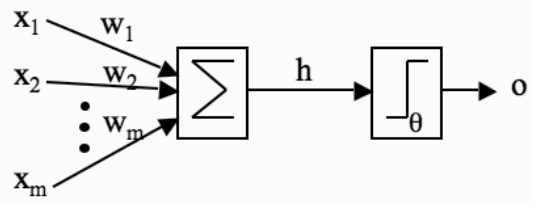
\includegraphics[scale=0.6]{plots/neuron.png}
 	\caption{McCullochs and Pitts' model of neutrons visualized. Image reproduced from \cite{Marsland} }
 	\label{fig:neuron}
 \end{figure}

The neurons are arranged in layers in the neural network, one visible layer that receives the input, and up to several hidden layers. The layers are arranged such that the output values from the visible nodes is the input values of the visible nodes. The nodes can also have bias values, that shift the output value $h$ with a certain number, and the nodes in different layers can be connected in different ways.  An example of a neural network with two layers is shown in figure \ref{fig:neural_network}.

 \begin{figure} [H]
	\centering
	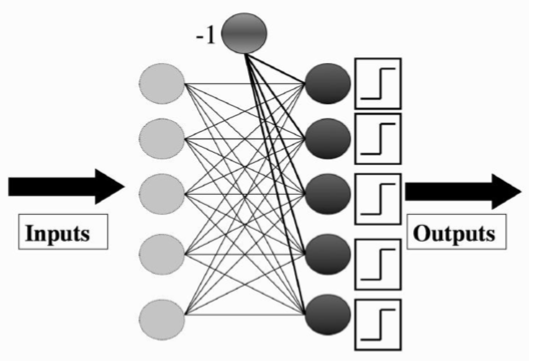
\includegraphics[scale=0.5]{plots/neural_network.png}
	\caption{An example of a neural network with one visible and one output layer of nodes, and with bias $-1$ on the hidden nodes. Image reproduced from \cite{Marsland} }
	\label{fig:neural_network}
\end{figure}

The idea behind machine learning is that the weights $W_i$, that decides how much a node puts emphazis on a given input, can be changed, and thus change the system's response to the same input. We will explain with the example from earlier, with huskies and the wolves: first, the program are shown pictures of wolves and huskies, and it is told the correct answer. The weights $W_i$ are then updated such that when a husky is shown, the output "husky" is generated, and the same for wolves. After a sufficiently long training period, the program's weights are optimalized for recognizing wolves and huskies. When shown a picture, the program should then by itself be able to determine wheter it is a wolf or a husky that it sees. 

\subsubsection{Restricted Boltzmann Machines} \label{sec:RBM}
There are plenty of ways to put together a neural network, as one can modify the number of nodes and layers, the bias, and also which nodes that are allowed to communicated. In this project, we will be using the so-called Restricted Boltzmann Machine (RBM). It is a two-layer network. The reason why it is named "restrictive" is that there are no connections between nodes in the same layer, but every node in the previous layer is connected to all the nodes in the next layer. The RBM can learn to draw samples from a probability distribution, which is just what we want in our project. In addition, we want to use a Gaussian-Binary RBM (see figure \ref{fig:RBM}), where the hidden nodes have binary values, while the positions of the particles can take continuous values, as they are, in fact, positions. 

\begin{figure}
\centering
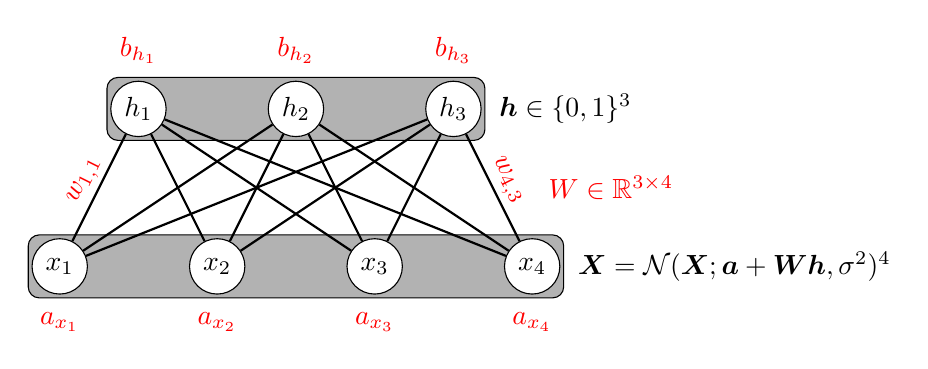
\begin{tikzpicture}[scale=2]
    % \draw ;
    \draw[fill=black!30, rounded corners] (-0.2, -0.2) rectangle (3.2, 0.2) {};
    \draw[fill=black!30, rounded corners] (0.3, 0.8) rectangle (2.7, 1.2) {};

    \node (v1)[neuron] at (0, 0) {$x_1$};
    \node (v2)[neuron] at (1, 0) {$x_2$};
    \node (v3)[neuron] at (2, 0) {$x_3$};
    \node (v4)[neuron] at (3, 0) {$x_4$};
    \node[right=0.1cm of v4] (v) {$\boldsymbol{X} = {\cal N}(\boldsymbol{X};\boldsymbol{a} + \boldsymbol{W} \boldsymbol{h}, \sigma^2)^4$};
    \node[learned,below=0.1cm of v1] (bv1) {$a_{x_1}$};
    \node[learned,below=0.1cm of v2] (bv2) {$a_{x_2}$};
    \node[learned,below=0.1cm of v3] (bv3) {$a_{x_3}$};
    \node[learned,below=0.1cm of v4] (bv4) {$a_{x_4}$};

    \node (h1)[neuron] at (0.5, 1) {$h_1$};
    \node (h2)[neuron] at (1.5, 1) {$h_2$};
    \node (h3)[neuron] at (2.5, 1) {$h_3$};
    \node[right=0.1cm of h3] (h) {$\boldsymbol{h} \in \{0, 1\}^3$};
    \node[learned,above=0.1cm of h1] (bh1) {$b_{h_1}$};
    \node[learned,above=0.1cm of h2] (bh2) {$b_{h_2}$};
    \node[learned,above=0.1cm of h3] (bh3) {$b_{h_3}$};

    \node[learned] (W) at (3.5, 0.5) {$W \in \mathbb{R}^{3 \times 4}$};

    \draw[learned,stateTransition] (v1) -- (h1) node [midway,above=-0.06cm,sloped] {$w_{1,1}$};
    \draw[stateTransition] (v1) -- (h2) node [midway,above=-0.06cm,sloped] {};
    \draw[stateTransition] (v1) -- (h3) node [midway,above=-0.06cm,sloped] {};

    \draw[stateTransition] (v2) -- (h1) node [midway,above=-0.06cm,sloped] {};
    \draw[stateTransition] (v2) -- (h2) node [midway,above=-0.06cm,sloped] {};
    \draw[stateTransition] (v2) -- (h3) node [midway,above=-0.06cm,sloped] {};

    \draw[stateTransition] (v3) -- (h1) node [midway,above=-0.06cm,sloped] {};
    \draw[stateTransition] (v3) -- (h2) node [midway,above=-0.06cm,sloped] {};
    \draw[stateTransition] (v3) -- (h3) node [midway,above=-0.06cm,sloped] {};

    \draw[stateTransition] (v4) -- (h1) node [midway,above=-0.06cm,sloped] {};
    \draw[stateTransition] (v4) -- (h2) node [midway,above=-0.06cm,sloped] {};
    \draw[learned,stateTransition] (v4) -- (h3) node [midway,above=-0.06cm,sloped] {$w_{4,3}$};

\end{tikzpicture}
\caption{An example of a Gaussian-Binary RBM with four visible nodes ($\boldsymbol{X}$) and three hidden nodes ($\boldsymbol{h}$), where $\boldsymbol{W}$ are the weights, and $\boldsymbol{a}$ and $\boldsymbol{b}$ are the bias weights. }
\label{fig:RBM}
\end{figure}

The joint probability distribution is known from statistical mechanics,
\begin{equation}
\label{eq:F_rbm}
F(\boldsymbol{X},\boldsymbol{H})=\frac{1}{Z}e^{-\beta E(\boldsymbol{X},\boldsymbol{H})}
\end{equation}
where we set $\beta=1/kT=1$ and $Z$ is the partition function, which can be ignored since it will vanish anyway. 

The system energy of a Gaussian-Binary RBM is given by
\begin{equation}
E(\boldsymbol{X},\boldsymbol{H})=\sum_{i=1}^{M}\frac{(X_i-a_i)^2}{2\sigma_i^2}-\sum_{j=1}^Nb_jH_j-\sum_{i,j=1}^{M,N}\frac{X_iW_{ij}H_j}{\sigma_i^2}
\end{equation}
\cite{Hinton}. We then define the NQS wave function as $\Psi = F(\boldsymbol{X},\boldsymbol{H})$, which has a general form of the probability distribution. In equation \ref{eq:wf_form} the form of the wave function is shown, when we have used that we have $M$ visible nodes and $N$ hidden nodes, and that the hidden nodes should take binary values. 

\begin{equation}
\label{eq:wf_form}
	\Psi = \frac{1}{Z} e^{\sum_i^M \frac{(X_i - a_i)^2}{2\sigma^2}} \prod_j^N (1+ e^{b_j + \sum_iM \frac{X_i W_{ij}}{\sigma^2}})
\end{equation}
See appendix C for derivation.

\subsection{Energy calculation} \label{sec:RBM_energy_cal}
We want to calculate the energy of the two-fermion system, given the wave function described in \ref{eq:wf_form}. As explained in \cite{Nordhagen}, the energy of the system is the expectation value of the Hamiltonian, but this is hard to compute directly. 

\begin{equation}
E_L(\boldsymbol{r})=\frac{1}{\Psi_T(\boldsymbol{r})}\hat{H}\Psi_T(\boldsymbol{r}).
\label{eq:Local_energy}
\end{equation}

By defining the local energy given in equation \ref{eq:Local_energy}, the energy can be expressed as equation \ref{eq:MC_energy}, and this can be solved with a Monte Carlo loop.

\begin{equation}
\label{eq:MC_energy}
E = \int | \Psi_T^2| E_L d\boldsymbol{r}
\end{equation}

\subsubsection{Exact energy for non-interacting case}

The wave function of one electron in a two-dimensional harmonic oscillator is given by

\begin{equation}
	\label{eq:one_e_wf_ho}
	\phi_{n_x, n_y} = A H_{nx} \sqrt{\omega} x H_{ny} \sqrt{\omega} y e^{-\frac{\omega(x^2 + y^2)}{2}}
\end{equation}
where $H_{nx} \sqrt{\omega} x$ is the Hermite polynomials and A is the normalization constant, and $n_x$ and $n_y$ are the principal quantum numbers. If we denote $\phi_1$ the spatial wave function for the first electron, and $\phi_2$ the spatial wave function for the second electron, then the total spatial wave function for the two-particle system is $\phi_1 \phi_2$. As explained in section \ref{sec:Presentation_of_potential}, the spin wave functions are anti-symmetric, and therefore it is fine that the spatial wave function is symmetric.

We know that the energy of a harmonic oscillator in one dimension is given by

\begin{equation}
	\label{eq:HO_energy}
	E_n = \omega (n + \frac{1}{2} )
\end{equation}
where $n$ is the principal quantum number.

For a one-electron system in two dimensions the energy can be shown to take the value 
\begin{equation}
H \ket{\phi_1} = E_1 \ket{\phi_1} = \omega(n_{x,1} + n_{y,1} + 1) \ket{\phi_1} \quad  \rightarrow E_1 = \omega(n_x + n_y + 1)
	\label{eq:exact_E_1P1D}
\end{equation}
where $n_x$ and $n_y$ are the principal quantum number for the $x$ and $y$ direction respectively, and we have used natural units, and thus all the energies are given in atomic units a.u.

When calculating the energy of the two-electron system we then get the following

\begin{equation}
	H \ket{\phi_1 \phi_2} = \ket{H \phi_1 } \ket{\phi_2} + \ket{\phi_1} \ket{H \phi_2} = E_1 \ket{\phi_1 \phi_2} + E_2 \ket{\phi_1 \phi_2} 
\end{equation}

For the ground state $n_x = n_y = 0$, $E_1 = E_2 = \omega$ and therefore the ground state energy is simply 

\begin{equation}
\label{eq:HO_energy_2omega}
	E_1 + E_2 = 2\omega.
\end{equation} 

For the non-interacting case with $\omega=1$ it is known the ground state energy is 3 a.u. \cite{Taut}. 

\subsection{Onebody density} \label{sec:onebody}
A quantity that often is handy to calculate is the onebody density. The onebody density is the density of particles in the potential, and may give a better understanding of the placement of the particles than their positions. The onebody density $\rho_i$ with respect to a given particle $i$ is given by equation \ref{eq:onebody_density}, which can be solved by Monte Carlo integration, as described in \cite{Nordhagen}.    

\begin{equation}
\label{eq:onebody_density}
\rho_i(\boldsymbol{r})=\int_{-\infty}^{\infty}d\boldsymbol{r}_1\hdots d\boldsymbol{r}_{i-1}d\boldsymbol{r}_{i+1}\hdots d\boldsymbol{r}_N |\Psi(\boldsymbol{r}_1,\hdots \boldsymbol{r}_N)|^2.
\end{equation}

Apart from the fact that the one body density is a good visual representation of the positions of the particles, it is also a quantity that is often calculated experimentally. Therefore, it is simpler to compare computational simulations to  experimental results when having calculated the onebody density.

Without interaction, the onebody density of particle $i$ is simply its wave function squared, which is known to be
\begin{equation}
\rho_i(\boldsymbol{r})=A^2e^{-\boldsymbol{r}_i^2}
\end{equation}
for a particle in the groundstate of a harmonic oscillator potential with $A$ as the normalization constant. Numerically we solve this by dividing the area around a particle into bins. Thereafter we count the number of particles in each bin, and divid by the area to get the density. The area of bin $k$ is
\begin{equation}
A_k=\pi r_k^2-\pi r_{k-1}^2=2\pi r_kdr-\pi dr^2
\end{equation}
where $r_k$ is the outer radius of bin $k$ and $dr$ is the bin width.

\subsection{Virial theorem} \label{sec:Virial_theorem}
The virial theorem is an equation in mechanics that gives a relation between the time-averaged kinetic energy $\langle T \rangle$ and the potential forces acting on $N$ particles confined in a stable system. The theorem takes the following form:

\begin{equation}
\langle T \rangle = - \frac{1}{2} \sum_{i=0}^N \langle \boldsymbol{F_i} \cdot \boldsymbol{r_i} \rangle 
\end{equation}

where $\boldsymbol{F_i}$ is the sum of forces acting on particle $i$.\par 
\vspace{3mm}

In a two-particle system where the potential is proportional to $r^n$, then the virial theorem simplifies to 

\begin{equation}
\label{eq:virial_simple}
2 \langle T \rangle = n \langle V_{tot} \rangle
\end{equation}

\subsection{Error estimation} \label{sec:error_estimation}
As a physicist one should always be sceptical to measurements presented without an estimation of the uncertainties. When someone says they have measured their height to be 1.90 cm, is the uncertainty $\pm 1 cm$ or $\pm 10 cm$? If they used $\pm 1 cm$, we have a fairly good idea of the height of the person, but if it is $\pm 10 cm$, we do not really know anything about the real height of the person. 
\par 
\vspace{3mm}
The error in a measurement is the difference between the true value of the measurand, $x$, and the measured value $x_i$:

\begin{equation}
	error = x - x_i
\end{equation}

However, the true value $x$ is rarely known. When $x$ is not known, it is thus impossible to give the error in the measurement. We must therefore be content with providing estimates of the error. It is common to give this uncertainty as the standard deviation $\sigma$; when performing a mesurement n times, such that we have n measured points $x_1, .., x_n$ where the average value is $ \langle x \rangle $, then the standard deviation is defined as

\begin{equation}
\label{eq:standard_dev}
\sigma_{\theta} =  \sqrt{\frac{1}{n-1} \sum_{k=1}^n (x_i - \langle x \rangle)^2}
\end{equation}

When giving the uncertainty, one writes $x_i \pm \sigma$, where $\sigma$ is so that $\approx 68 \%$ of the measured values lies within the interval $\pm \sigma$. 

There are different kinds of sources of error when conducting computer experiments. Systematic errors originate from faults in the theory used in the experiment, and this might give consistently wrong results. Systematic errors are hard to handle, as one might get seemingly good looking results. One way to avoid systematic results are to benchmark the code with either experimental results, or with other's computer simulation results. \par 
\vspace{3mm}
Another source of error is the statistical error, which is based on how many measurements you have done. In the example with the height measurement in the beginning of this section, if the experimentalist only measured the height one time, we can be fairly certain that this is not the true value of the person. If they, however, repeated the same measurement several times and then maybe used the average as the estimate of the measurand, we can be more confident that they have a better estimate, compared to when they only used one point. A common way to estimate the statistical uncertainty is with equation \ref{eq:variance_simplified}.

\begin{equation}
\label{eq:variance_simplified}
\sigma^2 \approx \langle x^2 \rangle - \langle x \rangle^2
\end{equation}

However, as explained in \cite{Nordhagen}, this does not account for the covariance between measurements. This leads to equation \ref{eq:variance_simplified} being an underestimation of $\sigma^2$, and is thus more a guideline for the size of the uncertainty, more than an actual estimate of it. Luckily, there are computational methods that can calculate $\sigma^2$ with the covariance contribution included. The method used in this project is the blocking method, presented in section \ref{sec:Blocking}.

\section{Method} \label{sec:Method}

\subsection{Variational Monte Carlo}
The Variational Monte Carlo method, often referred to as VMC, is a method in computational physics. The goal of VMC is to approximate the ground state energy of a quantum mechanical system by using the variational principle. The variational principle says that for any given trial wave function $\Psi_T$, the energy $E$ given this $\Psi_T$ is always more than or equal to the ground state energy $E_0$ of the system:

\begin{equation}
	\label{eq:variational_method}
	E = \frac{\bra{\Psi_T}H \ket{\Psi_T}}{\braket{\Psi_T}} \geq E_0
\end{equation} 

In VMC, the user inputs a trial wave function for the quantum mechanical system. Over a Monte Carlo loop, the particles in the system are moved randomly, and for each proposed move, the new position of the particle is accepted or rejected depending on whether the new position is more probable according to $\Psi_T$ or not, compared to the previous position. For the ground state wave function, the position which yields a minimum in the energy of the quantum mechanical system is the most probable position. The result is therefore that the particles in the system are moved towards lower energies. When the method has converged, the energy $E$ is an upper limit estimate of the true ground state energy $E_0$. If $\Psi_T$ in addition is the true ground state wave function, then $E=E_0$. 

\subsection{Metropolis algorithm}
Above, we described that the VMC method had to reject or accept proposed moves of the particles in the system. The task of handeling this is often left up to the Metropolis algorithm. The Metropolis algorithm uses the theory that the probability of a system to transition from a state $i$ to state $j$ is given by

\begin{equation}
W_{i\rightarrow j} = T_{i \rightarrow j}\cdot A_{i \rightarrow j}
\end{equation}
where $T_{i \rightarrow j}$ is the transition probability and $A_{i \rightarrow j}$ is the acceptance probability. If we denote the probability for being in a given state for $p$, and then look at the transition from a state $i$ to a state $j$ and back again, then it can be shown that we obtain the following relation between the transition and acceptance probabilities \cite{Nordhagen}:

\begin{equation}
\label{eq:metropolis_acceptance}
\frac{A_{j\rightarrow i}}{A_{i\rightarrow j}}=\frac{p_iT_{i\rightarrow j}}{p_jT_{j\rightarrow i}} = w
\end{equation}

As the Metropolis algorithm's job is to evaluate probable moves between states, the expression in equation \ref{eq:metropolis_acceptance} is used as the acceptance criteria. Thus the ratio $\frac{A_{j\rightarrow i}}{A_{i\rightarrow j}}$ describes if the system is more likely to move one way or the other. There are several methods that can be used for accepting and rejecting the moves, and these use different expressions for $T$ and $p$ in equation \ref{eq:metropolis_acceptance}. In this project, we will study the brute force and the Hastings sampling algorithms.

\subsubsection{Brute force}
The brute force got is name because when proposing and accepting moves, the algorithm does so without "thinking" which way the system will most probably move. A random particle with position $\boldsymbol{R}$ is chosen, and its new position $\boldsymbol{R}_{new}$ is proposed at random as follows:

\begin{equation}
\boldsymbol{R}_{new} = \boldsymbol{R} + \boldsymbol{r}\cdot \text{step}.
\end{equation}
where $\boldsymbol{r}$ is random numbers and $step$ is the steplength.
\par 
\vspace{3mm}
The brute force algorithm does not concider the transitions probabilities, and simply puts $T_{i\rightarrow j} = T_{j\rightarrow i}$. To check the probability of a system being found in a given state, it uses $p(\boldsymbol{R})=|\Psi_T(\boldsymbol{R})|^2$ for both position, such that the probability $w$ for the transition is given by

\begin{equation}
w=\frac{P(\boldsymbol{R}_{new})}{P(\boldsymbol{R})}=\frac{|\Psi_T(\boldsymbol{R}_{new})|^2}{|\Psi_T(\boldsymbol{R})|^2}.
\end{equation}

A random number $r \in [0,1]$ is then drawn, and compared to $w$. If $w$ is larger than $r$, then the new position is accepted, and if not, the move is rejected and the particle is moved back to its original position:

\begin{equation}
\text{New position: }
\begin{cases} 
\text{accept} & \text{if}\quad w > r \\
\text{reject} & \text{if}\quad w \leq r.
\end{cases}
\end{equation}

This way, the algorithm will over many iterations move the particles towards the most probable state.


\subsubsection{Metropolis-Hastings} \label{sec:Metropolis-Hastings}
The Metropolis-Hastings algorithm, also known as importance sampling, have a more refined approach to choosing new positions and accepting them, compared to the brute force method. Instead of proposing the new position at random, the Metropolis-Hastings algorithm considers the quantum force F, given by equation \ref{eq:drift_force}, which says something about which direction the particle is pushed in. 

\begin{equation}
\label{eq:drift_force}
\boldsymbol{F}(\boldsymbol{R}) = \frac{2 \nabla \psi_T(\boldsymbol{R})}{\psi_T(\boldsymbol{R})}
\end{equation}
The equation that describes the motion of a particle pushed around by the drift force $F$, is called the Langevin equation. The Langevin equation can be derived from the Fokker-Planch equation, which describes the time-evolution of the probability density function. The Langevin equation can be solved using the Euler method. The result, presented in equation \ref{eq:hastings_newpos} , describes how the Metropolis-Hastings algorithm chooses a new position for the random particle:

\begin{equation}
\label{eq:hastings_newpos}
R_{new} = R + DF(R)\Delta t + \xi\sqrt{\Delta t}
\end{equation}
where $D=\frac{1}{2}$ is the diffusion constant and $\Delta t$ is the timestep, that decides how long steps the method should take for each move. This is a much more educated guess compared to the brute force algorithm. 
\par 
\vspace{3mm}
When regaring the transition probabilities, the Metropolis-Hastings algoritm does not go the easy way with $T_{i\rightarrow j} = T_{j\rightarrow i}$.  Instead it uses that the transition probabilities are given as the Green's function, also found using the Fokker-Planch equation:

\begin{align}
G(R_{new},R,\Delta t)&=\frac{1}{(4\pi D\Delta t)^{3N/2}}\exp[-(R_{new} - R - D\Delta tF(R))^2/4D\Delta t]\notag\\
&=T_{R\rightarrow R_{new}}
\end{align}

such that the probability parameter $w$ becomes 

\begin{equation}
w = \frac{G(R,R_{new},\Delta t)|\Psi_T(R_{new})|^2}{G(R_{new},R,\Delta t)|\Psi_T(R)|^2}.
\end{equation}

Thereafter a random number $r$ is drawn and compared to $w$, just like in the brute force method. This more complicated way of proposing and accepting positions makes the Metropolis-Hastings slightly slower than the brute force method, but also quicker to converge towards the ground state. When using the Metropolis-Hastings algorithm, we need the expression for the quantum force for the NQS wave function. The calculations and the final expression of $\boldsymbol{F}$ are shown in appendix \ref{sec:appendix_A}.
\par 
\vspace{3mm}

One thing that is worth to note with the brute force and the Metropolis-Hastings algorithms when doing machine learning projects, is that both of them in this project are implemented so that only the positions, i.e., the visible nodes, are updated. This makes it so that we lose the opportunity to modify half of the system, which maybe yield a worse convergence than if we varied the whole system.


\subsection{Gibbs sampling}
As an alternative to the Metropolis algorithm, one can use the Gibbs sampling method. In both the brute force method and Metropolis-Hastings, one has to accound for that proposed particle moves can be rejected, and this "wastes" one Monte Carlo cycle with doing several flops, when no change is inflicted on the system. \par 
\vspace{3mm}
The Gibbs sampling algorithm differs from the Metropolis in several ways. In section \ref{sec:RBM} we wrote that we chose the trial wave function $\Psi = F(\boldsymbol{X},\boldsymbol{H})$, where $F$ is defined in equation \ref{eq:F_rbm}. In Gibbs sampling, we instead use the trial wave function $\Psi_T = \sqrt{F}$. 
\par 
\vspace{3mm}
Furthermore, instead of updating only the visible nodes, as is done in Metropolis, the Gibbs sampling algorithm is a two-step sampling process where first a new position is chosen, and then one of the hidden nodes are updated. The positions are sampled from a Gaussian probability distribution, shown in equation \ref{eq:gibbs_xsampling}, while the probability for sampling $h=1$ is shown in equation \ref{eq:gibbs_hsampling}.

\begin{equation}
\label{eq:gibbs_xsampling}
P(\boldsymbol{X} | \boldsymbol{h}) = \mathcal{N}(\boldsymbol{X}; \boldsymbol{a} + \boldsymbol{W} \boldsymbol{h}, \sigma^2)
\end{equation}

\begin{equation}
\label{eq:gibbs_hsampling}
P(H_j = 1 | \boldsymbol{X}) = \frac{1}{ 1 + e^{- b_j - \frac{\boldsymbol{X}^T \boldsymbol{W_{cols,j}} }{\sigma^2}}}
\end{equation}

When we say that the visible and hidden nodes here are "sampled", we mean that they are drawn from the probability distribution, and then automatically accepted. This is different from Metropolis, and should mean that the Gibbs sampling method converges faster than both brute force and Metropolis-Hansings, as no Monte Carlo cycles are lost on the move not being accepted. \par 
\vspace{3mm}
As we use a new trial wave function in Gibbs sampling, the expression for the local energy changes. The expression for the local energy using the Gibbs trial wave function is calculated in appendix \ref{sec:appendix_B}.


\subsection{Gradient descent}
We use stochastic gradient descent to update the weights in order to minimize the local energy. The process itself is quite similar to that one typically used in VMC where the weights are our variational parameters, but compared to a standard VMC we have a lot more parameters to vary. The updating algorithm for updating the variational parameter $\alpha_i$ goes as
\begin{equation}
\alpha_i^+=\alpha_i-\eta d\alpha_i
\end{equation}
where the gradient of the local energy with respect to parameter $\alpha_i$ is
\begin{equation}
d\alpha_i=\frac{\partial\langle E_L\rangle}{\partial \alpha_i}=2\bigg(\Big\langle E_L\frac{1}{\Psi}\frac{\partial\Psi}{\partial\alpha_i}\Big\rangle-\Big\langle E_L\Big\rangle\Big\langle\frac{1}{\Psi}\frac{\partial\Psi}{\partial\alpha_i}\Big\rangle\bigg)
\end{equation}
where $\eta$ is the learning rate. We need to do this for all the parameters, and for our purposes it is convenient to vectorize the gradient such that $d\boldsymbol{a}$ and $d\boldsymbol{b}$ are vectors and $d\boldsymbol{W}$ is a matrix. The gradients to implement are
\begin{equation}
d\boldsymbol{a}=\frac{1}{\Psi}\frac{\partial\Psi}{\partial\boldsymbol{a}}=\frac{\boldsymbol{X}-\boldsymbol{a}}{\sigma^2}
\end{equation}
\begin{equation}
d\boldsymbol{b}=\frac{1}{\Psi}\frac{\partial\Psi}{\partial\boldsymbol{b}}=\frac{1}{1+e^{-\boldsymbol{v}}}
\end{equation}
\begin{equation}
d\boldsymbol{W}=\frac{1}{\Psi}\frac{\partial\Psi}{\partial\boldsymbol{W}}=\frac{\boldsymbol{X}}{\sigma^2}\frac{1}{1+e^{-\boldsymbol{v}}}
\end{equation}
which means that we need to calculate $d\boldsymbol{b}$ and $d\boldsymbol{W}$ elementwise, i.e, $db_k=(1+e^{-v_k})^{-1}$. $\boldsymbol{v}$ is defined as
\begin{equation}
\boldsymbol{v}\equiv \boldsymbol{b} + \frac{\boldsymbol{X}^T\cdot\boldsymbol{W}}{\sigma^2}.
\end{equation}

\subsection{Blocking method} \label{sec:Blocking}
In section \ref{sec:error_estimation}, we described the need of a proper estimation of the uncertainty in computational simulations, where the covariance was included in the calculation od $\sigma$. A quick and easy way to get a proper estimate of the uncertainty, is by using the blocking method. If we have a data set ${x_1, x_2, ..., x_n }$ with $n$ data points, where the mean value is $\langle x \rangle$. We can calculate the standard deviation using equation \ref{eq:standard_dev}, however, as explained before, this does not include the covariance, as the data points ${x_1, x_2, ..., x_n }$  may be correlated.  A way to get around this, it by transforming the data set such that

\begin{equation}
x'_i = \frac{1}{2}(x_{2i} + x_{2i+1})
\end{equation}

The number of points in the transformed data set is now $n'$, and every $x'_i$ consists of two of the original data points. The transformed $x'_i$'s are referred to as blocks, and the standard deviation in each block $\sigma_i$ can now be calculated. An estimate of the total standard deviation $\hat{\sigma}$ when we have $n'$ transformed data points is

\begin{equation}
	\label{eq:total_std_dev}
	\hat{\sigma} = \frac{\sigma_1 + .. + \sigma_{n'}}{n'}
\end{equation} 

We now increase the block size, such that there are even more of the original data point in each block, and calculate the total standard deviation from equation \ref{eq:total_std_dev} again. If we continue doing this and plot the resulting estimates of $\hat{\sigma}$, we will observe that it first increases, until it flats out. When we have reached this plateu, we know that the data blocks $x'_i$ are no longer correlated. The covariance is then 0, and we have thus obtained a proper estimation of the uncertainty. 

\section{Code} \label{sec:Code}
In this section, we give an overview of the structure and implementation of our code, to make it easier for potential users to familiarize themselves with the code. 

\subsection{Structure}
In order to keep the code structured, we have split the running of the program up in several files. The user only needs to interact with main.cpp, as all the parameters for running the machine lerning project are set here. Examples are that the user can choose between brute force, Metropolis-Hastings og Gibbs sampling, and set the number of visible and hidden nodes, along with the number of iterations. main.cpp calls on the function GradientDecent in gradient\_decent.cpp, where the machine learning structure is implemented. The machine learning structure consists of the VMC-loop, where the nodes are updated, and the gradient decent method, where the weights are updated. GradientDecent uses the class WaveFunction in wavefunction.cpp to calculate the value of the wave function, along with the energy of the system. Depending on whether the user chose brute force, Metropolis-Hastings or Gibbs sampling, GradientDecent calls functions in either wavefunction.cpp, hastings\_tools.cpp or gibbs\_tools.cpp to update the positions and calculate the transition probabilities. The test functions are found in test.cpp. The structure can be seen in figure \ref{fig:program_structure}.

 \begin{figure} [H]
	\centering
	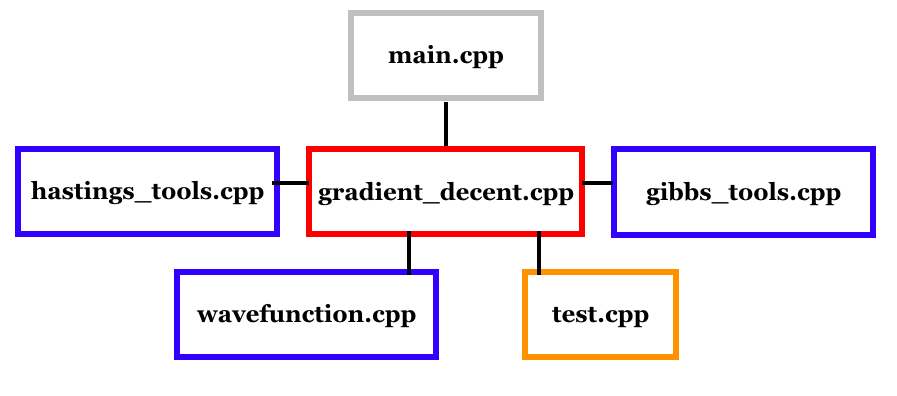
\includegraphics[scale=0.4]{program_structure.png}
	\caption{The structure of the machine learning program, showing the communication between the different files}
	\label{fig:program_structure}
\end{figure}

\subsection{Implementation}

\subsubsection{General implementation}
\lstset{basicstyle=\scriptsize}

\begin{lstlisting}
	Set up vectors X and h for visible and hidden nodes, fill with random numbers, X between -1 and 1, h with 0 and 1
	
	Set opp vectors a, b, W for the weights, fill with random numbers between -1 and 1
	
	Initialize class WaveFunction
	
	for iter iterations
		for MC Monte Carlo cycles
			#do VMC
		
		#do GradientDecent
		
		end when stopping criterias == true, when method has converged
		print final energy
\end{lstlisting}

\subsubsection{VMC}

\lstset{basicstyle=\scriptsize}
\begin{lstlisting}

for M Monte Carlo iterations
	
	if Metropolis:
		move random particle
		accept or reject move based on transition probability
		
	if Gibbs:
		sample new position and hidden node
		
	calculate energy of new position
	update sum of E_L

print estimated E 

\end{lstlisting}

\subsubsection{Gradient Decent}

\lstset{basicstyle=\scriptsize}
\begin{lstlisting}

for iter iterations:
	
	for MC Monte Carlo cycles:
		#do VMC
		
	Check if stopping criteria == true:
		if true, break and print final values
		
	Calculate gradient for the weights a, b and W
	Update a, b and W

\end{lstlisting}


\section{Results} \label{sec:Results}
Firstly, we calculate the energy of one particle in one dimension. Secondly, we extend the system to two interacting electrons in a two-dimensional harmonic oscillator. Furthermore the onebody densities with and without interaction are presented and finally we study how the total energy is distributed between kinetic energy and potential energy for various harmonic oscillator frequencies. 

\subsection{Energy calculations, without interaction}
We first study the energy of a non-interacting electron in one dimension, and in figure \ref{fig:energy1P1D} we compare the energies produced by the three methods as a function of number of iterations. 
 \begin{figure} [H]
 	\centering
 	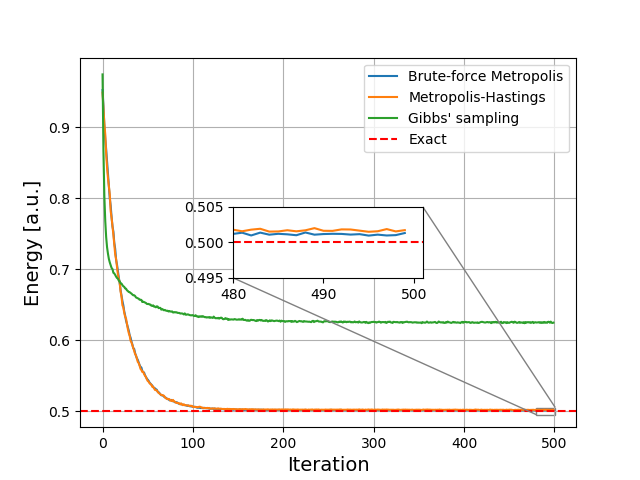
\includegraphics[scale=0.8]{plots/energy_comparison.png}
 	\caption{Energy as a function of number of iterations up to 500 iterations for one particle in one dimension. Brute-Force (BF) Metropolis (blue line), Metropolis-Hastings (MH) (orange line), Gibbs' (green line) and analytical value (dashed red line). All the samplings were conducted with MC=$2^{20}=1048576$, $\eta=0.01$, two hidden nodes, $\omega=1.0$ and $\sigma=1.0$. For BF we used steplength $dx=1.0$, while for MH the timestep was $dt=0.01$. See text for further description.}
 	\label{fig:energy1P1D}
 \end{figure}
We observe that the energies produced by brute-force and Metropolis-Hastings are very similar, and in fact it is hard to distinguish them. They also give lower energies to the analytical energy compared to Gibbs' sampling. In table \ref{tab:energies1P1D} some chosen energies from figure \ref{fig:energy1P1D} are listed, and we observe that brute-force has actually the smallest absolute error for all number of iterations. 

\begin{table} [H]
	\caption{Energy as a function of number of iterations up to 500 iterations for one particle in one dimension. \vspace{2mm}}
	\begin{tabularx}{\textwidth}{X|XXXX} \hline\hline
		\label{tab:energies1P1D}
		Iterations & BF & MH & Gibbs & Exact \\ \hline
				100 & 0.50633(23) & 0.50734(13) & 0.63524(89) & 0.5 \\
				200 & 0.50149(08) & 0.50232(36) & 0.62690(54) & 0.5 \\
				300 & 0.50136(03) & 0.50198(11) & 0.62562(52) & 0.5 \\
				400 & 0.50121(02) & 0.50198(07) & 0.62453(52) & 0.5 \\
				500 & 0.50132(02) & 0.50173(06) & 0.62471(52) & 0.5 \\ \hline
	\end{tabularx}
\end{table}

\subsubsection{Playing with learning rate and number of hidden nodes}
To find the lowest energy, we experiment with different learning rates and a various number of hidden nodes. We use brute-force Metropolis and in figure \ref{fig:compare_nodes} one can find energy plotted as  functions of number of iterations. Initially the energy is overall higher for more hidden nodes, but we get a closer energy to the exact energy for lower number of hidden nodes. 

 \begin{figure} [H]
 	\centering
 	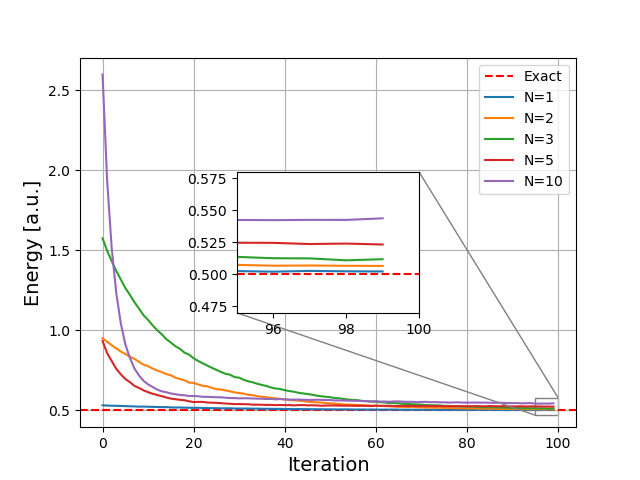
\includegraphics[scale=0.8]{plots/energy_compare_nodes.png}
 	\caption{Energy as functions of iterations for N=1,2,3,5 and 10. Brute-Force Metropolis is used, MC=5000000, $\eta=0.01$ and $dx=1.0$.}
 	\label{fig:compare_nodes}
 \end{figure}
 
Since the optimal number of hidden nodes is one in this case, we will use N=1 while optimizing the learning rate. In figure \ref{fig:compare_etas} we compare the energy convergence for various $\eta$'s.  Initially set all the weights and positions to 0.2, such that we they all start at the same point, and again we use brute-force Metropolis with $dx=1.0$.

 \begin{figure} [H]
 	\centering
 	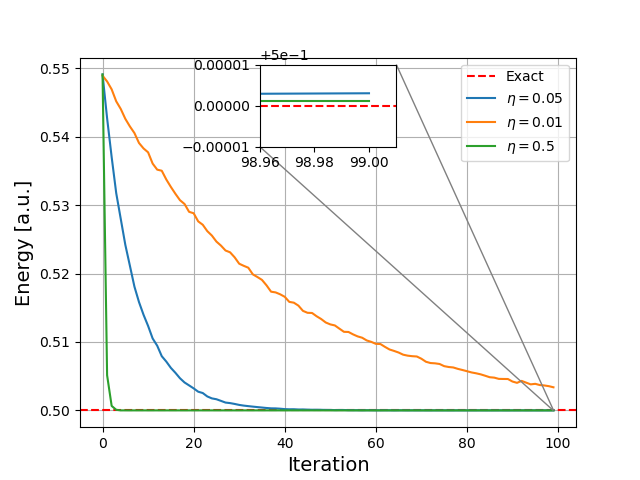
\includegraphics[scale=0.8]{plots/energy_compare_eta.png}
 	\caption{Energy as functions of iterations for $\eta$=1,2,3,5 and 10. Brute-Force Metropolis is used, MC=5e6, N=1 and $dx=1.0$.}
 	\label{fig:compare_etas}
 \end{figure}
The smaller learning rate the slower it converges, and after 100 iterations both $\eta$=0.5 and $\eta$=0.05 are really close to the exact value. 

\subsection{Energy calculations, with interaction}
We now go further to study the results from two iteracting fermions. 

 \begin{figure} [H]
 	\centering
 	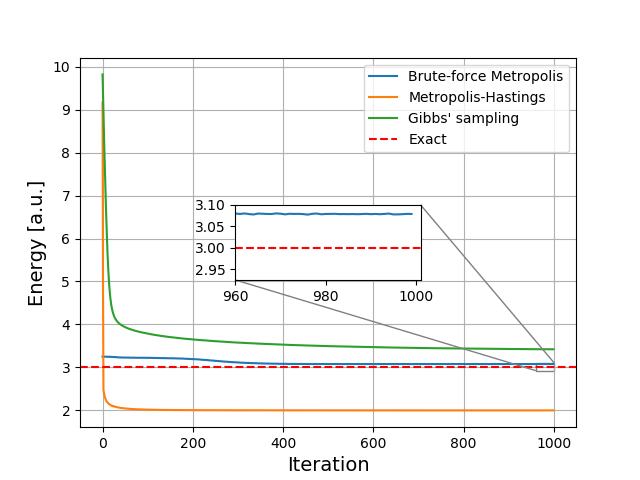
\includegraphics[scale=0.8]{plots/comparison_energy_2P.png}
 	\caption{Energy as a function of number of iterations up to 1000 iterations for two particles in two dimensions. Brute-Force Metropolis (blue line), Metropolis-Hastings (orange line), Gibbs' (green line) and analytical value (dashed red line). All the samplings were conducted with MC=$2^{25}=33 554 432$, $\eta=0.01$, two hidden nodes, $\omega=1.0$ and $\sigma=1.0$. For BF we used steplength $dx=1.0$, while for MH the timestep was $dt=0.01$. See text for further description.}
 	\label{fig:energy2P2D}
 \end{figure}

\begin{table} [H]
	\caption{Energy as a function of number of iterations up to 500 iterations for one particle in one dimension. \vspace{2mm}}
	\begin{tabularx}{\textwidth}{X|XXXX} \hline\hline
		\label{tab:energies2P2D}
		Iterations & BF & MH & Gibbs & Exact \\ \hline
				200 & 3.10897 & 3.10712 & 3.65337 & 3.0 \\
				400 & 3.08195 & 3.08410 & 3.52992 & 3.0 \\
				600 & 3.07979 & 3.07890 & 3.4714 & 3.0 \\
				800 & 3.07895 & 3.07970 & 3.44103 & 3.0 \\
				1000 & 3.07881 & 3.07791 & 3.42241 & 3.0 \\ \hline
	\end{tabularx}
\end{table}

\subsection{Onebody density}
In figure \ref{fig:OB} the onebody densities for two particles in two dimensions with and without interaction is plotted. From the energy calculations, we found Metropolis-Hastings method to be the better one for two particles, and henceforth we will therefore stick to it. 
 \begin{figure} [H]
 	\centering
 	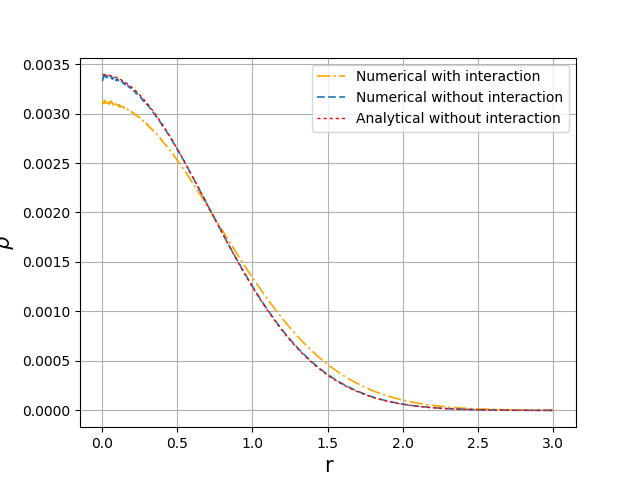
\includegraphics[scale=0.8]{plots/OB_comparison_MC_1e9.png}
 	\caption{Onebody densities plotted as a function of the distance from origin. The orange (dashed and dotted) represents the numerical calculation of two interacting particles, the blue (dotted) line represents the numerical calculation of two non-interacting particles, while the red (dotted) line repsresents the analytical calculation of two non-interacting particles. The graphs are normalized to 1 in the interval $r\in[0,3]$, and they are conducted in the way discussed in section \ref{sec:onebody}. We used 1000 bins, MC=1e9 Monte-Carlo cycles and the Metropolis-Hastings method.}
 	\label{fig:OB}
 \end{figure}
For the non-interacting case we see that the numerical calculation reproduces the analytical onebody density, but its slightly noisy for small $r$'s. The onebody density for two interacting fermions is broader and has a lower maximum.
 

\subsection{Average energies and distance}
In table \ref{tab:average_energies} average kinetic, interaction and potential energy is presented along with the mean distance for both the interacting and non-interacting case and for various frequencies. We observe that both the interaction energy and the potential energy increase as the frequency increase, while the mean distance decreases.

\begin{table} [H]
	\caption{In this table we present average kinetic ($\langle T\rangle$), interaction ($\langle V_{int}\rangle$) and external potential energies ($\langle V_{ext}\rangle$) for various $\omega$'s, along with the average distance between particles ($\langle |\boldsymbol{r}_i-\boldsymbol{r}_j|\rangle$) in the rightmost column. We used the brute-force Metropolis method with $dx=1.0$ and found the averages after convergence.  \vspace{2mm}}
	\begin{tabularx}{\textwidth}{c|XXXXX} \hline\hline
		\label{tab:average_energies}
		$\omega$ & $ E_{tot}$ [a.u.] & $\langle T\rangle$ [a.u.] & $\langle V_{ext}\rangle$ [a.u.] & $\langle V_{int}\rangle$ [a.u.] & $\langle |\boldsymbol{r}_i-\boldsymbol{r}_j|\rangle$ \\ \hline \\
				& \multicolumn{4}{c}{\textbf{Without interaction}}\\ \hline
				0.01 & 0.86104 & 0.86104 & 1.6997e-4 & - & 1.7483 \\
				0.05 & 0.86911 & 0.86410 & 0.0041111 & - & 1.6904 \\
				0.1 & 0.87778 & 0.86231 & 0.015474 & - & 1.6492 \\
				0.5 & 1.1947 & 0.91850 & 0.27619 & - & 1.3217 \\
				1.0 & 2.0004 & 0.98093 & 1.0195 & - & 1.2685 \\ \hline \\
		& \multicolumn{4}{c}{\textbf{With interaction}}\\ \hline
				0.01 & 1.1663 & 0.98781 & 9.4224e-4 & 0.17756 & 5.8220 \\
				0.05 & 1.2075 & 0.99888 & 0.021559 & 0.18710 & 5.5416 \\
				0.1 & 1.2736 & 0.98968 & 0.069086 & 0.21483 & 4.8911 \\
				0.5 & 2.0287 & 0.90810 & 0.56948 & 0.55025 & 2.4452 \\
				1.0 & 3.1638 & 0.92120 & 1.1673 & 1.0753 & 1.4412 \\ \hline
	\end{tabularx}
\end{table}


\section{Discussion} \label{sec:Discussion}
Initially we calculated the energy for one particle in one dimension to ensure that the method worked properly. Using equation \ref{eq:HO_energy} to calculate the ground state energy, we get that the energy for one particle in one dimention with $\omega=1$ should be $\frac{1}{2}$. The result of the calculation with the machine learning program with different sampling algorithms can be seen in figure \ref{fig:energy1P1D}. We see that both the  brute-force Metropolis and Metropolis-Hasting converges towards the analytical energy. Additionally, from table \ref{tab:energies1P1D}, we see that the variance decreases when the two methods converges towards $\frac{1}{2}$, as we increases the number of gradient decent cycles used in the minimalization. This is a good indication that our methods are approaching the correct value, even if we did not have an analytical anwer to compare them to. The two methods yield nearly identical results, while we would expect Metropolis-Hastings to be a better method, due to the more advanced sampling routine presented in section \ref{sec:Metropolis-Hastings}. However, the difference might be to small to give an impact to this project, as we use few particles.
\par 
\vspace{3mm}

From figure \ref{fig:energy1P1D}, one can see that Gibbs' sampling converges to a higher energy than the analytic value. The reason for that is probably related to how we define the wave function. For brute force and Metropolis-Hastings, we use the probability distribution defined in $\ref{eq:F_rbm}$ to represent the wave function, while the wave function used in Gibbs' sampling is the square root of the probability distribution. It seems this representation of the wave function is further away from the true wave function, and thus Gibbs converges towards a higher energy. This is in accordance with the variational principle; a worse guess on trial wave function will yield a upper bound estimate of the ground state energy $E$ that is larger than the true ground state energy $E_0$.

\par 
\vspace{3mm}
For the case where the Coulomb repulsion is turned on, the results of the convergence of the Metropolis algorithms and the Gibbs sampling method are shown in figure \ref{fig:energy2P2D} and table \ref{tab:energies2P2D}. Again, as described above, we see that the brute force and Metropolis-Hastings algorithms converges towards the exact value of $3$ a.u, while Gibbs sampling approaches a higher energy. The fraction of deviation between the calculated and analytical value is roughly the same for the interacting and non-interacting case for all three methods, which can be seen by comparing table \ref{tab:energies1P1D} and \ref{tab:energies2P2D}.

\par 
\vspace{3mm}
We varied the number of hidden nodes $N$ used in the machine learning program, as seen in figure \ref{fig:compare_nodes}. We see that varying the number of hidden nodes changes the rapidness of the method's convergence. For few hidden nodes, the convergence of the energy seems to happen slower, while for many hidden nodes, it decends steeply towards the analytical energy. \textcolor{red}{This can maybe be explained by when there are more free parameters that can be varied, the optimalization occurs faster. $\rightarrow$ Discuss with Vilde}. \par 
We also see that we get better estimates of the ground state energy when using fewer hidden nodes. This is as expected, since more hidden nodes means more variables that has to be updated for each cycle, and thus a less precise answer. \textcolor{red}{$\rightarrow$ Discuss with Vilde}.\par
The results discussed above are run for the non-interacting case with the brute force Metropolis algorithm, but the interacting case yielded the same results, and we therefore found them unnecessary to include. 
\par 
\vspace{3mm}

Furthermore, we observed the effects of changing the learning rate $\eta$ used in the gradient decent method. The results are shown in figure \ref{fig:compare_etas}. We see that the convergence rapidness was heavily dependent on the learning rate, where a low learing rate gave a slow convergence. This is what we expected, as the learning rate defines how much the weights $W$, $a$ and $b$ are updated in each gradient decent iteration, that is, how large steps the method takes for each iteration. Larger steps will lead to the method aproaching the convergence more rapidly. As seen in this figure, if we limit the number of gradient decent iterations, then the choice of $\eta=0.01$ has not converged by the end of 100 minimalization iterations. A good choice of $\eta$ is thus necessary for the method to work optimally.
\par  
\vspace{3mm}

The onebody density calculated for two particles in two dimentions with the Metropolis-Hastings method is plotted in figure \ref{fig:OB}. We are able to reproduce the analytical onebody density without interaction. When interaction is introduced, the distribution of particles becomes broader and lower. This is explained by the two electrons now being supject to a repulsive force which pushed them apart, so that the average distance between the electrons increases. This creates a broader onebody density distribution.
\par 
\vspace{3mm}

In table \ref{tab:average_energies}, we see that the estimates of the average distance between the two electrons $\langle |\boldsymbol{r}_i-\boldsymbol{r}_j|\rangle$ increases with increasing harmonic oscillator frequancy $\omega$. This is as expected, as the higher $\omega$, the steeper the sides of the potential well, and thus the electrons are forced together. We also observe that the average distance for the same $\omega$ increases when the interaction is turned on, which as explained above, correspons to the Coulomb repulsion forcing the electrons apart.
\par 
\vspace{3mm}

As explained in section \ref{sec:Virial_theorem}, the virial theorem holds for particles in stable systems, and the relation between the time-averaged kinetic and potential energy for potentials that are proportional to $r^n$ is shown in equation \ref{eq:virial_simple}. In the non-interacting case, the only potential affecting the particles is the harmonic oscillator potential, which is proportional to $r^2$. Thus equation \ref{eq:virial_simple} gives that the time-averaged kinetic and potential energies should be equal. From table \ref{tab:average_energies}, we see that we are able to reproduce this for two particles without interaction and $\omega=1.0$. However, for different values of $\omega$, it seems that the method becomes unstable, and we are no longer able to reproduce the virial theorem. In the interaction case, both the harmonic oscillator potential and the Coulomb interaction contributes to the total potential, and the total potential is thus no longer on the form $r^n$. Thus the simple relation between the time-averaged kinetic and potential energies in equation \ref{eq:virial_simple} no longer applies.
\par 
\vspace{3mm}

Another concern regarding table \ref{tab:average_energies} is that the energies in the non-interacting case are not on the form $2 \omega$, as they should have been, accoring to equation \ref{eq:HO_energy_2omega}. This is likely due to the same unstability described above, which makes us unable to reproduce the virial theorem. 

\section{Conclusion} \label{sec:Conclusion} 
In this project, we have found that by using principles of machine learning in combination with Variational Monte Carlo, we are able to find good upper bound estimates of the ground state energy in a system consisting of two electrons in a harmonic oscillator. The brute force Metropolis and Metropolis-Hastings yields nearly identical results, while Gibbs sampling gives higher estimates of $E_0$, due to a different choice in trial wave function. 
\par 
\vspace{3mm}
The choice of learning rate $\eta$ and number of hidden nodes $N$ used in the simulation affects the convergence rate and final results, where the convergence rate is higher for more hidden nodes and higher  $\eta$. 
\par 
\vspace{3mm}
The onebody density distribution obtained in this project maches the analytical calucaltion for the non-interacting case. The distribution becomes broader and lower when turning on the interaction, which matches the physical explanation that the repulsive Coulomb force forces the particles apart.
\par
\vspace{3mm}
We are solely able to reproduce the virial theorem for $\omega=1.0$, as the code becomes unstable for different choices of $\omega$.


\newpage

\section{Appendix A - Local energy and quantum force calculations for Metropolis} \label{sec:appendix_A}

\subsection{Local energy}

The energy can be calculated by introducing a local energy, where the acerage local energy goes to the true energy with a sufficient amount of samples, as explained in \ref{sec:Theory}. This local energy can be splitted up in a kinetic part, a part from the harmonic oscillator potential and a interacting part,
\begin{equation}
E_L=\sum_{k=1}^{M}(E_{\text{KIN},k} + E_{\text{EXT},k})+E_{\text{POT}}.
\end{equation}
As discussed in \cite{Nordhagen}, the kinetic part can be expressed as
\begin{align}
E_{\text{KIN},k}&=\frac{1}{\Psi_T}\nabla_k^2\Psi_T\\
&=(\nabla_k\ln\Psi_T)^2+\nabla_k^2\ln\Psi_T
\end{align}
where we have used that
\begin{equation}
\frac{1}{\Psi_T}\nabla_k\Psi_T=\nabla_k\ln\Psi_T.
\end{equation}

\begin{equation}
\frac{\partial}{\partial X_k}\ln\Psi_T=-\frac{X_k-a_k}{\sigma^2}+\sum_{j=1}^{N}\frac{W_{kj}}{\sigma^2}\text{Logistic}(v(j))
\end{equation}
\begin{equation}
\frac{\partial^2}{\partial X_k^2}\ln\Psi_T=-\frac{1}{\sigma^2}+\sum_{j=1}^{N}\frac{W_{kj}^2}{\sigma^4}\text{Logistic}^2(v(j))e^{v(j)}
\end{equation}
where 
\begin{equation}
\text{Logistic}(x)=\frac{1}{1+e^x}
\end{equation}
and
\begin{equation}
v(j)=b_j+\sum_{i=1}^{M}\frac{X_iW_{ij}}{\sigma^2}.
\end{equation}
Thus the local energy can be expressed as
\begin{align}
E_L&=\sum_{i=1}^{N}\frac{\boldsymbol{W}_{*i}^T\boldsymbol{W}_{*i}}{\sigma^4}\text{Logistic}^2\big(v(i)\big)\\
&\phantom{=}+\sum_{i,j=1}^{N,N}\frac{\boldsymbol{W}_{*i}^T\boldsymbol{W}_{*j}}{\sigma^4}\text{Logistic}\big(v(i)\big)\text{Logistic}\big(v(j)\big)\\
&\phantom{=}-2\sum_{i=1}^N\frac{\boldsymbol{W}_{*i}^T(\boldsymbol{X}-\boldsymbol{a})}{\sigma^4}\text{Logistic}(v(i))\\
&\phantom{=}+\frac{(\boldsymbol{X}-\boldsymbol{a})^T\cdot(\boldsymbol{X}-\boldsymbol{a})}{\sigma^4}-\frac{M}{\sigma^2}+\boldsymbol{X}^T\boldsymbol{X}+E_{\text{INT}}
\end{align}

\subsection{Quantum force}
In equation \ref{eq:drift_force}, the equation for the quantum force is given, but we repeat it here:

\begin{equation*}
\label{eq:drift_force}
\boldsymbol{F}(\boldsymbol{R}) = \frac{2 \nabla \psi_T(\boldsymbol{R})}{\psi_T(\boldsymbol{R})}
\end{equation*}

 When implementing importance sampling, we need the expression for the quantum force for the NQS wave function. As shown above, 
 
\begin{equation}
\frac{1}{\Psi_T}\nabla_k\Psi_T=\nabla_k\ln\Psi_T.
\end{equation}

and

\begin{equation}
\frac{\partial}{\partial X_k}\ln\Psi_T=-\frac{X_k-a_k}{\sigma^2}+\sum_{j=1}^{N}\frac{W_{kj}}{\sigma^2}\text{Logistic}(v(j))
\end{equation}

The expression for the quantum force is thus

\begin{equation}
\boldsymbol{F}(\boldsymbol{R})=-2\frac{X_k-a_k}{\sigma^2}+2\sum_{j=1}^{N}\frac{W_{kj}}{\sigma^2}\text{Logistic}(v(j))
\end{equation}



\section{Appendix B - Gibbs local energy and gradient calculation} \label{sec:appendix_B}

\subsection{Local energy}
We need the expression for the local energy with the new trial wave function $\Psi_T = \sqrt{F(\boldsymbol{X}, \boldsymbol{H})}$. We denote this new wave function $\Psi ^* = \sqrt{\Psi}$. Earlier, we saw that we had the following relation:

\begin{equation}
\frac{1}{\Psi_T}\nabla_k^2\Psi_T = (\nabla_k\ln\Psi_T)^2+\nabla_k^2\ln\Psi_T
\end{equation}

Using $\Psi ^* = \sqrt{\Psi}$, we now get

\begin{align}
	\frac{1}{\Psi ^*}\nabla_k^2\Psi ^*
	&= (\nabla_k \ln \Psi ^*)^2 + \nabla_k^2 \ln \Psi ^* \\
	&= (\nabla_k \ln \Psi^{\frac{1}{2}})^2 + \nabla_k^2 \ln \Psi^{\frac{1}{2}} \\
	&= \frac{1}{4}(\nabla_k\ln\Psi_T)^2 + \frac{1}{2}\nabla_k^2\ln\Psi_T
\end{align}

We see that there are two constants which differ the local energy caculated with $\Psi$ and $\Psi ^*$. 

\subsection{Gradient for gradient decent method}
When calculating the gradients for $\boldsymbol{W}$, $\boldsymbol{a}$ and $\boldsymbol{b}$ when using the wave function $\Psi ^* = \sqrt{\Psi}$, we must remember that:

\begin{equation}
	\nabla \ln \Psi^{\frac{1}{2}} = \frac{1}{2} \nabla \ln \Psi
\end{equation}

We thus get a factor $2$ difference in the gradients that are used to uptade the weights $\boldsymbol{W}$, $\boldsymbol{a}$ and $\boldsymbol{b}$, which we must remember to add when running Gibbs sampling.

\section{Appendix C - Derivation of the wave function}
We have seen that the probability of having a set of positions $\boldsymbol{X}$ with a set of hidden nodes $\boldsymbol{h}$ is given by
\begin{equation}
F(\boldsymbol{X},\boldsymbol{H})=\frac{1}{Z}e^{-\beta E(\boldsymbol{X},\boldsymbol{H})}
\end{equation}
where we set $\beta=1/kT=1$, $Z$ is the partition function and $E(\boldsymbol{X},\boldsymbol{h})$ is the system energy
\begin{equation}
E(\boldsymbol{X},\boldsymbol{H})=\sum_{i=1}^{M}\frac{(X_i-a_i)^2}{2\sigma_i^2}-\sum_{j=1}^Nb_jH_j-\sum_{i,j=1}^{M,N}\frac{X_iW_{ij}H_j}{\sigma_i^2}
\end{equation}
such that
\begin{equation}
F_{\text{RBM}}(\boldsymbol{X},\boldsymbol{h})=e^{\sum_{i=1}^M \frac{(X_i - a_i)^2}{2\sigma^2}} e^{\sum_{j=1}^N\Big(b_jh_j+\sum_{i=1}^M\frac{X_iW_{ij}}{\sigma^2}\Big)}.
\end{equation}
We skip the partition function because it will not affect the results (it is just a normalization constant). The probability of a set of positions only is therefore the sum over all sets of $\boldsymbol{h}$, $\{\boldsymbol{h}\}$:
\begin{align}
F_{\text{RBM}}(\boldsymbol{X})&=\sum_{\{\boldsymbol{h}\}}e^{\sum_{i=1}^M \frac{(X_i - a_i)^2}{2\sigma^2}} \prod_{j=1}^Ne^{b_jh_j+\sum_{i=1}^M\frac{X_iW_{ij}h_j}{\sigma^2}}\notag\\
&=\sum_{h_1}\sum_{h_2}\hdots\sum_{h_N}e^{\sum_{i=1}^M \frac{(X_i - a_i)^2}{2\sigma^2}}\cross\notag\\
&\phantom{=}e^{b_1h_1+\sum_{i=1}^M\frac{X_iW_{i1}h_1}{\sigma^2}}e^{b_2h_2+\sum_{i=1}^M\frac{X_iW_{i2}h_2}{\sigma^2}}\hdots e^{b_Nh_N+\sum_{i=1}^M\frac{X_iW_{iN}h_N}{\sigma^2}}\notag\\
&=e^{\sum_{i=1}^M \frac{(X_i - a_i)^2}{2\sigma^2}}\prod_{j=1}^N\sum_{h_j=0}^1e^{b_jh_j+\sum_{i=1}^M \frac{X_i W_{ij}h_j}{\sigma^2}}\notag\\
&=e^{\sum_{i=1}^M \frac{(X_i - a_i)^2}{2\sigma^2}} \prod_j^N (1+ e^{b_j + \frac{\boldsymbol{X}^T\boldsymbol{W}_{*j}}{\sigma^2}})
\end{align}


\newpage
\section{References}

\begingroup
\renewcommand{\section}[2]{}
\begin{thebibliography}{}
	\bibitem{MHJ15}
	Morten Hjorth-Jensen.
	Computational Physics 2: Variational Monte Carlo methods, Lecture Notes Spring 2018.
	Department of Physics, University of Oslo,
	(2018).
	\bibitem{Marsland}
	S. Marsland, \emph{Machine Learning: An algorithmic Perspective, Second edition} (2015)
	\bibitem{Nordhagen}
	 D. Gjestvang, E. M. Nordhagen \emph{Computational Physics II: Project 1} (2018)
	 \bibitem{Project2}
	 V. Flugsrud and M. Hjort-Jensen
	 Project 2, The restricted Boltzmannn machine applied to the quantum many body problem. Deadline June 1
	 Department of Physics, University of Oslo,
	 (2018).
	\bibitem{Taut}
	 M. Taut \emph{Two electrons in an external oscillator potential: Particular analytic solutions of a Coulomb correlation problem.} Phys. Rev. \textbf{A 48}, 3561 (1993).
	 \bibitem{Carleo}
	 G.Carleo and M. Troyer  \emph{Solving the quantum many-body problem with artificial neural networks} Science 355, Issue 6325, pp. 602-606 (2017)
	 \bibitem{Chilton}
	 A. Chilton \emph{The Properties and Applications of Quantum Dots} (2014) \url{https://www.azoquantum.com/Article.aspx?ArticleID=31} downloaded May 6th 2018
	 \bibitem{Hinton}
	 G.E. Hinton \emph{A Practical Guide to Training Restricted Boltzmann Machines}, Lecture Notes in Computer Science, vol \textbf{7700}. Springer, Berlin, Heidelberg (2012)

	
	
\end{thebibliography}
\endgroup

\end{document}
